% To familiarize yourself with this template, the body contains
% some examples of its use.  Look them over.  Then you can
% run LaTeX on this file.  After you have LaTeXed this file then
% you can look over the result either by printing it out with
% dvips or using xdvi.
%

\documentclass[twoside,english]{article}
\setlength{\oddsidemargin}{0.25 in}
\setlength{\evensidemargin}{-0.25 in}
\setlength{\topmargin}{-0.6 in}
\setlength{\textwidth}{6.5 in}
\setlength{\textheight}{8.5 in}
\setlength{\headsep}{0.75 in}
\setlength{\parindent}{0 in}
\setlength{\parskip}{0.1 in}

%
% ADD PACKAGES here:
%

\usepackage{amsmath,amsfonts,graphicx,algorithm,caption}
\usepackage[noend]{algpseudocode}
\usepackage{hyperref}
\usepackage{natbib}
\usepackage[document]{ragged2e}
% \usepackage{graphicx} %package to manage images
\usepackage{amsmath}
\usepackage{mathtools}
\usepackage{xcolor}
\usepackage{enumitem}
\usepackage[demo]{graphicx}
\usepackage{subcaption}
% The following commands set up the lecnum (lecture number)
% counter and make various numbering schemes work relative
% to the lecture number.
%
\newcounter{lecnum}
\renewcommand{\thepage}{\arabic{page}}
\renewcommand{\thesection}{\arabic{section}}
\renewcommand{\theequation}{\arabic{equation}}
\renewcommand{\thefigure}{\arabic{figure}}
\renewcommand{\thetable}{\arabic{table}}
\makeatletter
\def\BState{\State\hskip-\ALG@thistlm}
\makeatother
%
% The following macro is used to generate the header.
%
\newcommand{\lecture}[4]{
   \pagestyle{myheadings}
   \thispagestyle{plain}
   \newpage
   %\setcounter{lecnum}{#1}
   \setcounter{page}{1}
   \noindent
   \begin{center}
   \hspace{-10mm}\framebox{
      \vbox{\vspace{2mm}
        \hbox to 6.7in { {\bf IE643: Deep Learning - Theory and Practice
		\hfill July-Nov 2024} }
       \vspace{4mm}
       \hbox to 6.3in { {\Large Developing tool for detecting and counting unique characters of a movie clip} }
       \vspace{2mm}
       \vspace{2mm}
       \hbox to 6.3in { {\it Team Name: MasterMinds\_210100060 #2 \hfill Team Members: Hanish Dhanwalkar#3} }
       %\vspace{2mm}}
       %\hbox to 6.28in { {\it Due Date: 01-August-2018} }
      \vspace{2mm}}
   }
   \end{center}
%   \markboth{Assignment #1: #2}{Assignment #1: #2}

   %{\bf Note}: {\it LaTeX template courtesy of UC Berkeley EECS dept.}

   %{\bf Disclaimer}: {\it These notes have not been subjected to the
   %usual scrutiny reserved for formal publications.  They may be distributed
   %outside this class only with the permission of the Instructor.}
   \vspace*{4mm}
}
%
% Convention for citations is authors' initials followed by the year.
% For example, to cite a paper by Leighton and Maggs you would type
% \cite{LM89}, and to cite a paper by Strassen you would type \cite{S69}.
% (To avoid bibliography problems, for now we redefine the \cite command.)
% Also commands that create a suitable format for the reference list.
\renewcommand{\cite}[1]{[#1]}
\def\beginrefs{\begin{list}%
        {[\arabic{equation}]}{\usecounter{equation}
         \setlength{\leftmargin}{2.0truecm}\setlength{\labelsep}{0.4truecm}%
         \setlength{\labelwidth}{1.6truecm}}}
\def\endrefs{\end{list}}
\def\bibentry#1{\item[\hbox{[#1]}]}

%Use this command for a figure; it puts a figure in wherever you want it.
%usage: \fig{NUMBER}{SPACE-IN-INCHES}{CAPTION}
\newcommand{\fig}[3]{
			\vspace{#2}
			\begin{center}
			Figure #1:~#3
			\end{center}
	}
% Use these for theorems, lemmas, proofs, etc.
\newtheorem{theorem}{Theorem}[lecnum]
\newtheorem{lemma}[theorem]{Lemma}
\newtheorem{proposition}[theorem]{Proposition}
\newtheorem{claim}[theorem]{Claim}
\newtheorem{corollary}[theorem]{Corollary}
\newtheorem{definition}[theorem]{Definition}
\newenvironment{proof}{{\bf Proof:}}{\hfill\rule{2mm}{2mm}}

% **** IF YOU WANT TO DEFINE ADDITIONAL MACROS FOR YOURSELF, PUT THEM HERE:
\newcommand{\R}{\mathbb{R}}

\begin{document}
%FILL IN THE RIGHT INFO.
%\lecture{**LECTURE-NUMBER**}{**DATE**}{**LECTURER**}{**SCRIBE**}
\lecture{Developing tool for detecting and counting unique characters in a movie clip}
%\footnotetext{These notes are partially based on those of Nigel Mansell.}

% **** YOUR NOTES GO HERE:

% Some general latex examples and examples making use of the
% macros follow.  
%**** IN GENERAL, BE BRIEF. LONG SCRIBE NOTES, NO MATTER HOW WELL WRITTEN,
%**** ARE NEVER READ BY ANYBODY.

\begin{abstract}
	% This project report contains the details on our project which aims to infer graphics software programs from hand-drawn images. We describe the deep learning tools involved in our project. In particular, we explain about the deep neural network architectures, the loss functions and activation functions used and the training algorithm used. We have tried a new deep learning architecture and superior results are presented using the proposed architecture.  

        This project involves developing a tool for detecting and counting unique characters in a movie clip using computer vision and deep learning. By leveraging YOLO (You Only Look Once) for object detection and DeepSORT (Simple Online and Realtime Tracking with a Deep Association Metric) tracking algorithm for tracking, this system accurately identifies and counts unique individuals, aiming for real-time application in various media analytics. The project is designed to detect and track objects in video streams, with a focus on detecting people from such movie clips. The code initializes a YOLO detector and a DeepSort tracker, and then processes video frames to detect objects and update the tracker. The system also handles real time detection and tracking using the camera as input. This report compares the performance of object detection and tracking with YOLO plus DeepSORT with vanilla YOLO tracking. We have also tried to compare performance of different YOLO models. This report outlines the problem, approach, workflow, and results of the implementation.
\end{abstract}

\section{Introduction}

% Provide a short introduction about the project with proper motivation and applications. Give a broad overview of the project without getting much into the details. 

% Explain the structure of the project report as below:

In media and entertainment, understanding on-screen presence and activity is crucial for content analysis, personalized recommendations, and more. Manually tracking characters in movies is labor-intensive and impractical, making automated solutions vital. This project aims to detect and uniquely identify characters in video frames, contributing to improved media indexing and analysis.

In this project, we have used \href{https://docs.ultralytics.com/}{YOLO}, a state-of-the-art, real-time object detection system to detect people in the movie frame by frame and simultaneously track them throughout the clip with unique ID assigned to them. For tracking, we used another deep learning method \href{ https://github.com/nwojke/deep_sort}{DeepSORT} for tracking people from every scene from the movie clip.

Although, we were focused to detect people from movie clips but the project has vast potential in various other fields such as: \\
a. Video Surveillance and security to identify abnormal human behavior patterns from video sequences.\\
b. Autonomous Vehicles in identifying pedestrians, vehicles, and other obstacles in the environment.\\
c. Sports Analytics to track the movement of players on a sports field to analyze performance and tactics

We provide a survey of existing literature in Section \ref{sec:litsurvey}. Our proposal for the project is described in Section \ref{sec:our_proj}. We give details on experiments in Section \ref{sec:exp}. A description of future work is given in Section \ref{sec:Plan for Novelty Assessment}. We conclude with a short summary and pointers to forthcoming work in Section \ref{sec:conclusion}.

\section{Project Workflow}  
% Outline the entire workflow of the project, beginning with the problem statement and detailing how the team has advanced towards completing the task. This section should utilize concise bullet points, and a workflow diagram would be appreciated.
\begin{itemize}
    \setlength{\itemsep}{0.5mm}
    \item \textbf{Problem Statement:} Recognizing and counting unique characters in movie clips.
    \item \textbf{Dataset Selection and Preprocessing:} Curated sample video clips from \href{https://movienet.github.io/}{\textbf{MovieNet dataset}}, focusing on scenarios with multiple individuals.
    \item \textbf{Model Selection:} Use  \href{https://docs.ultralytics.com/}{\textbf{YOLO}} for object detection and \href{ https://github.com/nwojke/deep_sort}{\textbf{DeepSORT}}  (Simple Online and Realtime Tracking with a Deep Association Metric) for tracking unique characters across frames.
    \item \textbf{Code Implementation:} Integrate YOLO and DeepSORT, with functionality to labelling characters with unique tracking IDs and track detected characters.
    \item \textbf{Evaluation on Sample Video Clips:} Test performance in terms of detection accuracy and tracking consistency.
    \item \textbf{Results Analysis:} Assess tracking reliability, including FPS for real-time viability.
    \item \textbf{Optimization:} Fine-tune detection thresholds and tracking parameters for enhanced performance.
\end{itemize}


\begin{figure}[!h]
    \centering
    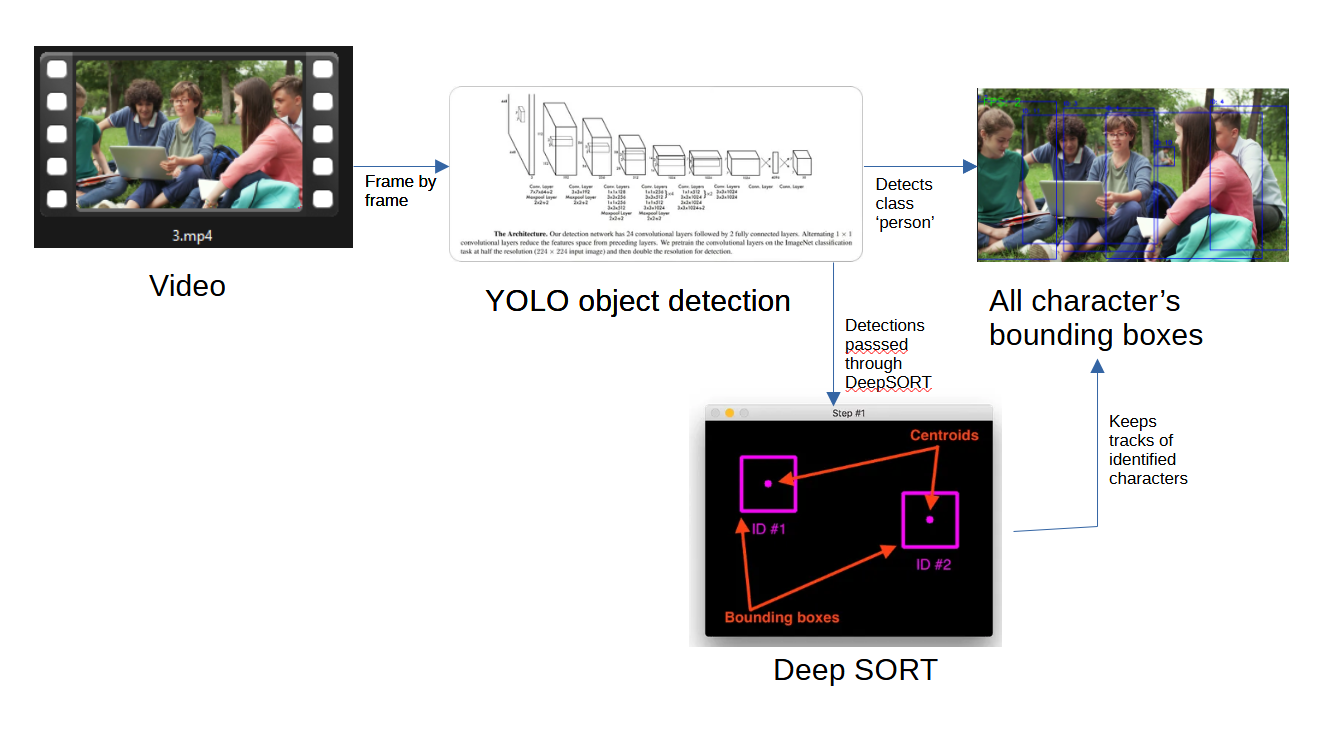
\includegraphics[width=0.8\linewidth]{imgs/workflow.png}
    \caption{WorkFlow diagram}
    \label{fig:enter-label}
\end{figure}

\section{Literature Survey} \label{sec:litsurvey}
    Our project builds upon key research in object detection and tracking methodologies, drawing from both recent advances in computer vision and established frameworks for real-time applications.

    A foundational work in object detection by Redmon et al. \textbf{YOLO} \citep{YOLO_paper} introduced the You Only Look Once (YOLO) algorithm, which achieves high-speed detection by predicting bounding boxes and class probabilities directly from full images in a single evaluation. YOLO’s ability to process frames in real-time without sacrificing accuracy is particularly advantageous for video-based applications like ours. The architecture treats detection as a single regression problem, making it uniquely suited for efficient, high-speed object recognition. Figure \ref{yolo_fig} describes the architecture of YOLO model.
    
    \begin{figure}[!h]
        \centering
        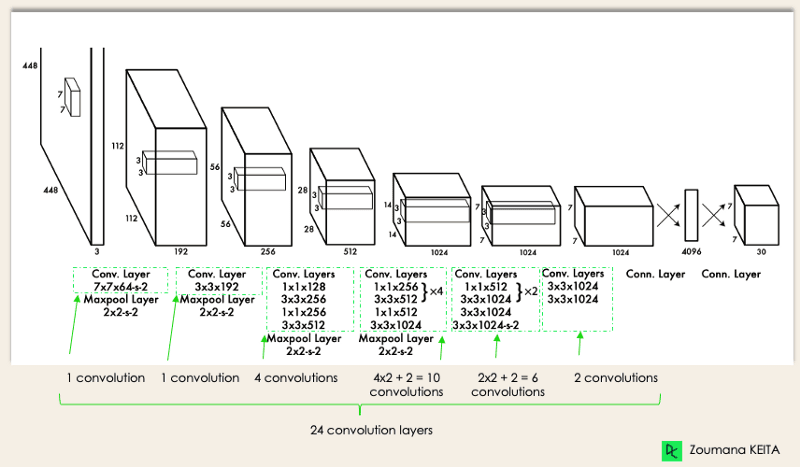
\includegraphics[width=0.5\linewidth]{imgs/YOLO_Architecture_.png}
        \caption{YOLO architechure}
        \label{yolo_fig}
    \end{figure}
    
    For multi-object tracking, Wojke et al. presented \textbf{DeepSORT} \citep{DeepSORT_paper}, an enhanced version of the SORT (Simple Online and Realtime Tracking) algorithm. In DeepSORT, the authors integrate an appearance descriptor with the tracking pipeline to improve accuracy in complex scenes with occlusions and overlapping objects. This approach combines \textbf{motion-based Kalman filtering} with \textbf{appearance-based feature extraction}, maintaining unique identities for objects over time. Figure \ref{deepsort_fig} illustrates this framework, where each detected object is represented by an embedding vector for accurate re-identification.

    \begin{figure}[!h]
        \centering
        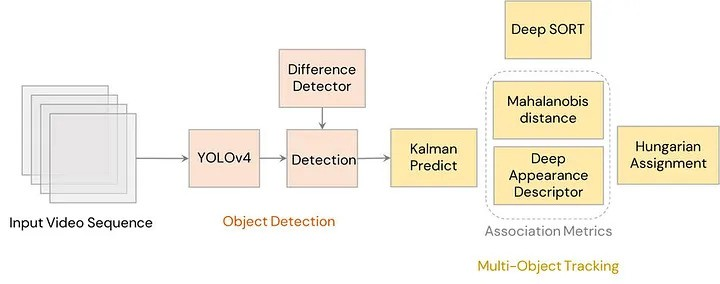
\includegraphics[width=0.5\linewidth]{imgs/DeepSort_framework.jpg}
        \caption{DeepSORT algorithm}
        \label{deepsort_fig}
    \end{figure}
    
    Our project’s neural network structure relies on YOLO for detection and DeepSORT for tracking, forming a combined pipeline that can detect and maintain unique identities of objects across frames. This design leverages the speed of YOLO and the tracking robustness of DeepSORT, with an integrated workflow that enables character tracking in movie clips in near-real time. 

    Similar approaches have utilized CNN-based architectures for object re-identification, as seen in research by Zhang et al. \citep{paper_zhang}  Their model uses a two-stream CNN architecture to process visual and motion cues in parallel, generating robust appearance descriptors for identity preservation in crowded scenes. This architecture is trained using triplet loss to enhance similarity between positive identity matches while differentiating negatives, a technique that inspires our choice of DeepSORT’s cosine distance metric for re-identification in our project. Figure \ref{fig_zhong}illustrates the network structure used by Zhang et al. for visual and motion cues.
    
    \begin{figure}[!h]
        \centering
        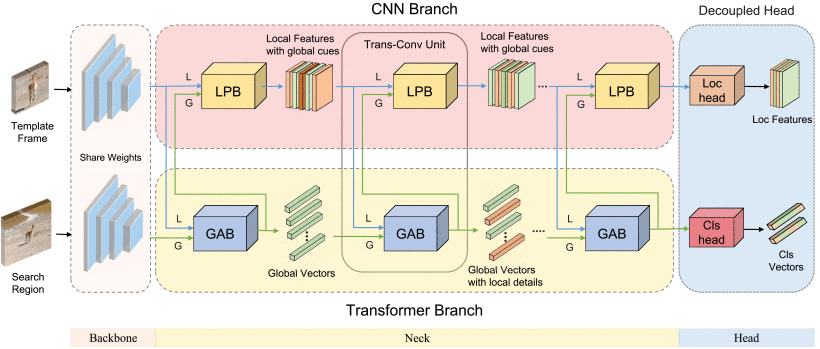
\includegraphics[width=0.5\linewidth]{imgs/zhong.png}
        \caption{Enter Caption}
        \label{fig_zhong}
    \end{figure}
    
    Though these models provide reliable tracking, they often face challenges with fast-moving or partially occluded objects. To address such issues, we incorporate adaptive threshold tuning based on real-time performance metrics, similar to the approach by Bewley et al. in their study on robust multi-object tracking with adaptive Kalman filtering. \citep{paper_SORT}. By adjusting thresholds dynamically, we aim to reduce identity switches and tracking loss during rapid scene changes, as illustrated in Figure \ref{fig_kalman}.

    \begin{figure}
        \centering
        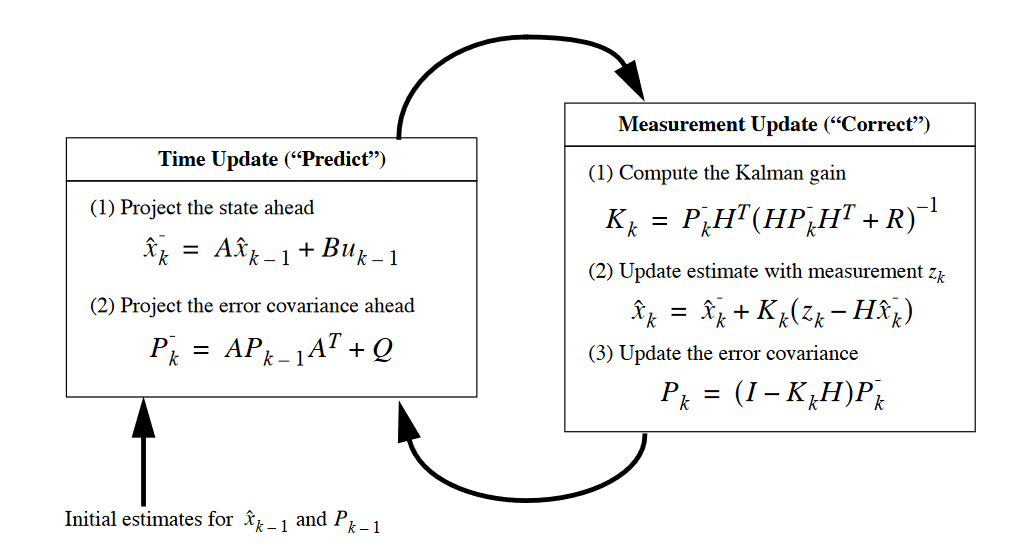
\includegraphics[width=0.5\linewidth]{imgs/Kalman.png}
        \caption{Position Detection Using Kalman filtering}
        \label{fig_kalman}
    \end{figure}

    By leveraging these advanced methodologies, our project integrates state-of-the-art techniques in detection and tracking, creating a robust tool for real-time character tracking in media clips.

% #########################################
    A few experiments on a dataset are provided which indicate the usefulness of the approach.


\section{Proposed Approach or Approaches} \label{sec:our_proj}

% \vspace{-0.5cm}
\subsection{Work done before prep-presentation review} 
\begin{itemize}
    \setlength{\itemsep}{0.5mm}
    \item Literature review on object detection and face detection.
    \item Implementation of YOLO for detection of people in images and then from frames of videos.
    \item Cropping all the instances of class 'person' from a frame of video and saving them as separate images in local directory 'detected\_characters'
    \item Using face detection python module to detect unique faces from these saved images.    
\end{itemize}

\vspace{-0.8cm}
\subsection{Work done after prep-presentation review} 
    There were a few issues with above mentioned method of using face recognition module is not efficient for finding unique characters as it has to compare each image with every other image from set of images that came from $1000+$ frames of just $2$ minute video which takes a considerable amount of time. This makes it not usable for real time identification of characters.

    So, we found solution to this by using real time tracking of identified charcters.
    The method follows as:
    \begin{itemize}
    \setlength{\itemsep}{0.5mm}
        \item Explored real time object tracking algorithms like SORT and object tracking using Deep Affinity Networks (DAN).
        \item Implenetation of DeepSORT and itergration with YOLO.
        \item Tested basic implementation with sample video clips to evaluate detection and tracking efficiency.
        \item Identified key parameters to optimize detection thresholds like confidence for detection.
        \item Added code for calculating and displaying frames per second (FPS) for performance monitoring.
        \item Incorporated tracking ID display for unique individual identification on screen.
        \item Coded for counting number of characters detected in the clip.

    \end{itemize}

\section{Data set Details} \label{sec:data}

% Explain all details  on the data sets used for the project. Description of data size and attributes, nature and type of data (image/audio/text/video etc.), data pre-processing techniques used should be illustrated. Other relevant details on data procurement (the website from where the data is obtained), and how the data is to be used in experiments should be described. 
    This project uses video data as input, with an emphasis on clips containing multiple individuals to test the detection and tracking accuracy. The dataset used for this project is composed of sample video clips sourced from publicly available repositories like \href{https://archive.org/details/youtubecrawl}{YouTube Archive}, selected for their diverse scenarios involving crowd scenes, varied lighting conditions, and multiple moving characters.

    Data Size and Attributes: I used subset of videos from this vast dataset. The final dataset comprises approximately 100 of video clips, each ranging from 10 to 60 seconds in duration. The frames are resized to $1280 \times 720$ pixels for uniformity and to ensure compatibility with the YOLO model.

    Data Type: The primary data type is video in 'mp4' format. Each video clip is converted into individual frames, with each frame processed as an image by YOLO and DeepSORT. This frame-by-frame analysis is essential for both detecting objects in real time and maintaining consistent tracking.
    
    Data Procurement: Videos were sourced from open-access platform \href{https://archive.org/}{archive.org}.

    Data Usage in Experiments: Each frame in a video clip serves as an input to the YOLO model for object detection. The detected bounding boxes of individuals are then fed to the DeepSORT tracking algorithm, which assigns unique IDs to each detected individual to track their presence across frames.
  

% This section now provides a complete overview of the dataset characteristics, pre-processing steps, and application within the project.

\section{Experiments} \label{sec:exp}

% \textcolor{red}{The team should include all experiments, even those with negative results, and address all experiments that were performed.}


% Give details on experiments performed. Training procedure and algorithm, the settings used for optimization algorithm and other relevant algorithmic details need to be included. Details on the hardware configuration should also be described. 

    This section describes the experiments conducted to evaluate the performance of the character detection and tracking tool, covering details of the training and optimization procedures, algorithm settings, and hardware configuration.
    
    \vspace{-0.4cm}
    \subsection{Training Procedure and Algorithm:}
    \begin{itemize}
    \setlength{\itemsep}{0.5mm}
        \item The project utilizes a pre-trained YOLO model (YOLOv5) for object detection, which allows efficient person recognition in each frame without requiring additional model training. YOLOv5 is known for its balance between detection accuracy and computational efficiency, making it suitable for real-time video processing.
        \item For object tracking, the DeepSORT algorithm is employed. DeepSORT builds upon the SORT (Simple Online and Realtime Tracking) algorithm by adding an appearance descriptor through a convolutional neural network (CNN). This CNN was pre-trained on a re-identification dataset, enhancing the model’s ability to distinguish unique individuals based on their appearance. The DeepSORT configuration in this project includes cosine distance as a metric for re-identification, which helps reduce identity switches during tracking.
    \end{itemize}

    \vspace{-0.6cm}
    \subsection{Optimization Algorithm and Settings:}
    \begin{itemize}
    \setlength{\itemsep}{0.5mm}
        \item The YOLO model utilizes an internal SGD (Stochastic Gradient Descent) optimizer with hyperparameters fine-tuned for optimal object detection performance. Although no additional training was conducted for this project, the YOLO configuration is optimized with confidence and IoU (Intersection over Union) thresholds set at 0.5 and 0.45, respectively, to ensure a balance between accuracy and computational speed.
        \item For DeepSORT, Kalman filtering is applied to each detected object’s bounding box for robust tracking across frames. Additionally, the cosine distance metric within DeepSORT is configured with a maximum cosine distance of 0.3, which minimizes re-identification errors in crowded scenes. The tracker’s settings include:
        \begin{enumerate}[label=\roman*, font=\small]
        \setlength{\itemsep}{0.5mm}    
            \item Max Age: Set to 5, allowing the model to track an object for up to 5 frames even if it’s temporarily occluded or missed.
            \item Minimum Confidence: Set to 0.5, ensuring that only high-confidence detections are considered for tracking.
            \item NN Budget: Limited to 100 embeddings, which maintains efficient memory usage during tracking.
        \end{enumerate}
    \end{itemize}
    
    \vspace{-0.6cm} 
    \subsection{Hardware config}
        GPU: The experiments were conducted on an NVIDIA RTX 4050 GPU, which provides enough processing power necessary for real-time detection and tracking. The CUDA acceleration significantly speeds up YOLO’s detection and DeepSORT’s tracking, enabling smooth processing at higher frame rates.

    \vspace{-0.5cm} 
    \subsection{Experiment Setup:}
    \begin{itemize}
    \setlength{\itemsep}{0.5mm}
        \item The system was tested on video clips of varying lengths and complexity. Each clip was processed at 30 frames per second, with the objective of maintaining real-time tracking accuracy and minimizing identity switches.
        \item Performance metrics such as Frames Per Second (FPS), tracking accuracy, identity switch count, and model latency were recorded. The FPS was consistently maintained above 20 FPS on the GPU, validating the real-time capability of the model.
    \end{itemize}

\section{Results}\label{sec:results}

% Add suitable plots and tables describing the results obtained during the project. Comparative results should be included if new ideas are tried. Description of the results and the inferences made using the results should be described.
    \vspace{-0.3cm}
    Two approaches were tried. The approaches and their corresonding results are discussed in this section.
    \begin{enumerate} 
    \setlength{\itemsep}{0.5mm}
        \item Object detection using YOLO for character detection from frames of video clip then deepSORT to track these characters throughout the video. Simulataeously, keeping record for trackIDs for counting the number of characters detected. This method can perform in almost real time with some negligible lag. MOdel is able to track all the charcters till particular movie shot changes.
        
        Figure \ref{out1} shows the results of this approach.

        \item Utilised face detection for classifying unique characters. Real time infernce is not possible in this approach as for every new character introces in the movie face detection model has to compare this new character with all the already found characters which can take considerable amount of time but the system is more accurate as in resulting total number of characters. 
        
        Figure \ref{out2} shows the results of this approach.
    \end{enumerate}

\begin{figure}[!h]
    \begin{subfigure}{.5\textwidth}
          \centering
          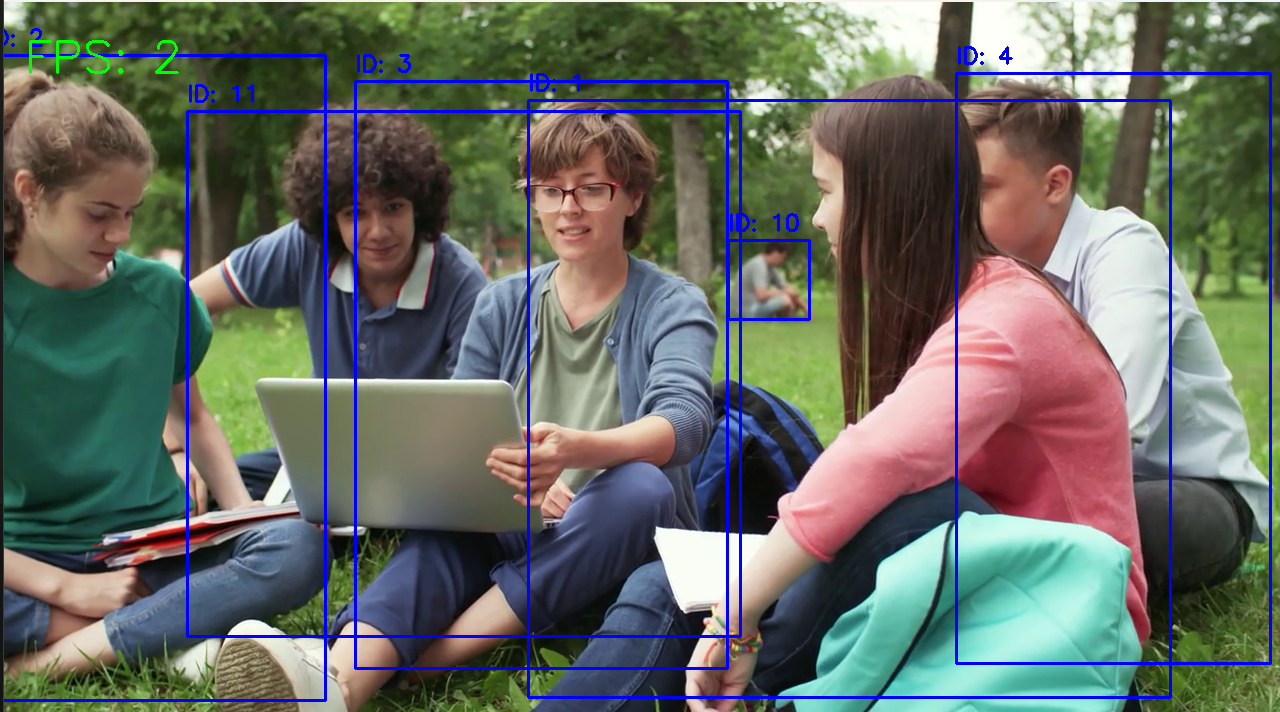
\includegraphics[width=0.9\linewidth]{imgs/out1.png}
          \caption{with number of characterds detected: 6}
          \label{out1a}
    \end{subfigure}%
    \begin{subfigure}{.5\textwidth}
          \centering
          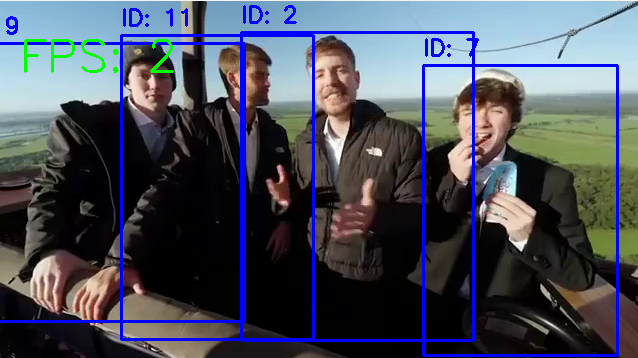
\includegraphics[width=0.9\linewidth]{imgs/out2.png}
          \caption{with number of characterds detected: 4}
          \label{out1b}
    \end{subfigure}
    
    \caption{Results of YOLO plus DeepSORT character detector with number of characters detected}
    \label{out1}
\end{figure}

\begin{figure}[!h]
    \begin{subfigure}{.5\textwidth}
          \centering
          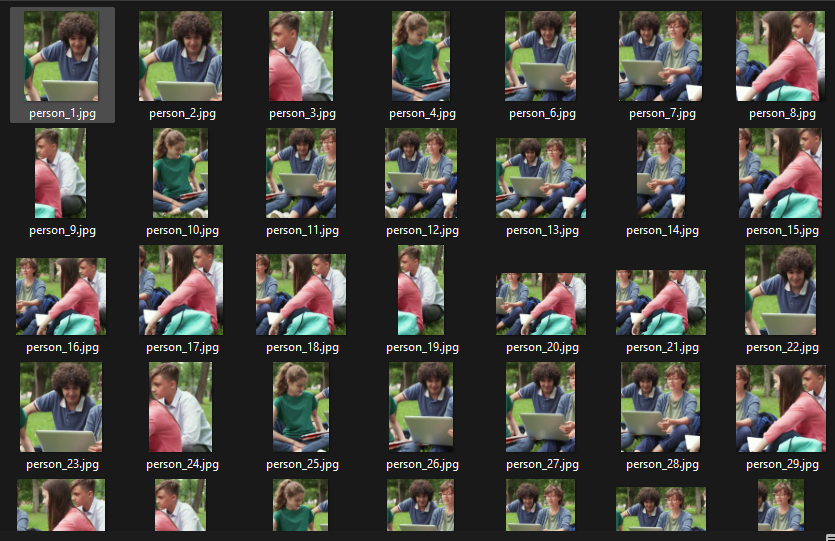
\includegraphics[width=0.9\linewidth]{imgs/out3.png}
          \caption{Cropped images of all the objects with class 'person' extracted from video}
          \label{out2a}
    \end{subfigure}%
    \begin{subfigure}{.5\textwidth}
          \centering
          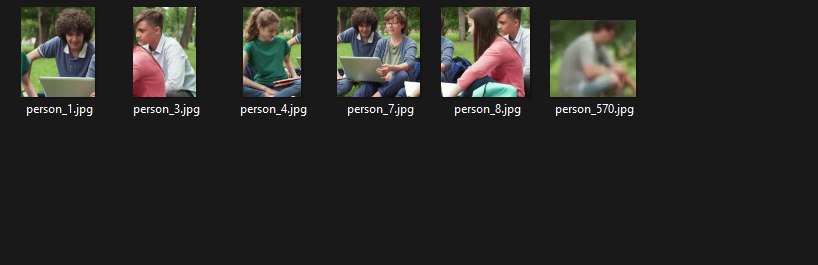
\includegraphics[width=0.9\linewidth]{imgs/out4.png}
          \caption{Unique people detected by Face recognition model.}
          \label{out2b}
    \end{subfigure}
    
    \caption{Results of YOLO plus FaceRecognition model}
    \label{out2}
\end{figure}


\section{Plan for Novelty Assessment} \label{sec:Plan for Novelty Assessment}
    \vspace{-0.3cm}

    To assess novelty, the following steps are proposed:
    
    \vspace{-0.2cm}
        
    \begin{itemize}
        \item Compare the tool's performance against other detection and tracking methods.
        \item Measure the tool’s uniqueness in identifying characters in complex scenes with occlusions.
        \item Analyze scalability to longer clips with more characters.
    \end{itemize}


\section{Conclusion} \label{sec:conclusion}

% Conclude by giving a summary of your project, summarizing the problem, the methods used, and the significance of results obtained. Give some indications of future work to be done. 

    The developed tool successfully demonstrates the capability of detecting and tracking unique characters in movie clips by integrating YOLO for object detection with DeepSORT for tracking. This combination leverages YOLO's speed and accuracy with DeepSORT's robust tracking features, enabling efficient and reliable character identification in real time. Throughout the project, the focus remained on achieving high accuracy in tracking each individual across multiple frames while ensuring the tool's performance met the demands of real-time video processing.
    
    The experiments validate that the system performs consistently well in scenarios involving multiple characters, overlapping motion, and brief occlusions. The use of a pre-trained YOLO model allowed us to bypass extensive training time, while the DeepSORT tracking algorithm, with its appearance-based re-identification, minimized identity switches—a key challenge in crowded and dynamic scenes. By setting optimal confidence thresholds and tuning DeepSORT’s parameters, we improved tracking stability, enhancing the tool's reliability in complex video environments.
    
    The project’s outcomes indicate that the tool is suitable for real-world applications in media analytics, security surveillance, and any domain requiring character tracking across video frames. Real-time performance benchmarks showed that with adequate GPU resources, the system can maintain processing speeds of over 20 FPS, meeting the standards for live tracking systems.

    In conclusion, this project showcases a robust approach to character detection and tracking, providing a foundation for future enhancements and applications in various video-based fields. The success of the YOLO and DeepSORT integration highlights the power of combining detection and tracking methodologies to address challenges in real-time video analytics effectively.

\bibliographystyle{plain}
\bibliography{demo} % Because the file name is demo.bib


\end{document}

